\documentclass[12pt,english,frenchb,letterpaper]{article}
\usepackage[T1]{fontenc}
\usepackage[utf8]{inputenc}
\usepackage{geometry}
\usepackage{setspace}
\usepackage{graphics}
\usepackage{graphicx}
\usepackage{amsmath,amssymb,amsfonts,textcomp}
\usepackage{color}
\usepackage{calc}
\usepackage{verbatim}
\usepackage{longtable}
\geometry{verbose, letterpaper,tmargin=3cm,bmargin=3cm,lmargin=3cm,rmargin=3cm}
\usepackage[french]{babel}


% Custom commands for the report
\newcommand{\action}[3] {
\begin{tabbing}
\textit{Action}\=\textit{(#1)},\\
\> PRECOND: 
     #2 
     \\
\> EFFECT: \textit{#3} .\\
\end{tabbing}}



\begin{document}
\thispagestyle{empty}
\begin{center}
{\large\em GEI790:  Intelligence Artificielle formelle}
\vfill
Rapport de l'App 1\\
présenté à l'équipe professorale de S8\\
\vfill
par:\\
Alexandre Malo\hspace{2cm} 05 659 076\\
Erick Lavoie\hspace{2cm} 05 646 456\\
\vfill
Date: \today
\end{center}

\newpage
\onehalfspacing


\tableofcontents

\newpage


\section{Introduction}
% Alex
% 0.5 page
Ce rapport présente les résultats de recherches pour l'amélioration de l'intelligence de joueur informatisés (\textit{JI}).
Les \textit{JI} qui évoluent entourés de joueurs humains font face à un problème critique. En fait, ils ne possèdent pas une intelligence suffisante afin de s'adapter aux multiples situations imprévisibles des humains. De plus, les \textit{JI} sont trop prévisible et rendent les jeux rapidement monotones. À ce jour, l'amélioration de \textit{JI} est l'élément le plus crucial pour une évolution saine de la compagnie.

Pour répondre à ce problème, l'ingénieur en chef a déterminé l'utilisation de méthodes d'intelligence artificielle. Les recherches effectuées comportent plusieurs volets afin de s'assurer de répondre aux besoins réels de la majorité de nos jeux à plateforme multijoueurs. Voici les études qui ont été réalisées:

\textbf{Méthode de recherches}
\begin{enumerate}
 \item Non informé
 \item Informé avec heuristique
\end{enumerate}

\textbf{Méthode de planification}
\begin{enumerate}
 \item recherche par espaces d'états
 \item partiellement ordonnée
\end{enumerate}

Avec une représentation de l'intelligence artificielle en logique de premier ordre, il devient très facile de réutiliser les algorithmes d'IA pour une multitude de jeux différents. Avec cette généralisation possible, les recherches ont été effectuées et testées dans l'environnement de jeux \textit{BlockBlitz}. Cette particularité rend la recherche sur les méthodes de l'intelligence artificielle intéressante afin de réduire le coût de développement de tous les jeux dans la compagnie. L'implémentation des algorithmes a toute été réalisée à l'aide du langage prolog afin d'accélérer le développement. Ce dernier est un langage qui est entièrement basé sur la logique du premier ordre.

Il existe en fait plusieurs autres techniques d'intelligence artificielle que celles présentées précédemment. C'est pourquoi qu'en plus de ces recherches, une analyse sommaire de méthodes plus évoluées est aussi présentée. À la fin de ce rapport se trouves toutes les recommandations à utiliser pour résoudre l'incapacité actuelle des \textit{JI}.


\section{Recommandation et justification de la technique de planification}
% Erick
% 3 pages
L'analyse des différentes techniques de planification a permis de faire ressortir les éléments suivants.  Cependant, étant donné que le choix de la technique de planification est indépendant du choix de la technique de recherche qui l'implémente, ces deux sujets seront traités séparément.

\subsection{Techniques de planification}
Dans les deux cas,il s'agit de trouver une séquence d'action qui permet d'atteindre un but. Dans le cas de la planification de la recherche par espace d'état, la recherche s'effectue sur l'état de l'environnement de jeu alors que dans le cas de la planification partiellement ordonnée, la recherche s'effectue sur l'environnement d'actions, c'est-à-dire les actions et leur dépendance mutuelles. 

\subsubsection{Planification par recherche d'espace d'état}

La planification par recherche d'espace d'état est la plus simple à mettre en oeuvre puisqu'elle est conceptuellement très similaire au comportement de l'agent dans la situation réelle.  Il s'agit en quelque sorte d'essayer différents plans possibles et d'observer l'évolution de l'environnement pour chacun de ces plans jusqu'à ce que l'on obtienne l'état désiré.  Il est possible de faire la recherche par chaînage avant ou arrière en s'appuyant sur les préconditions et les effets des différentes actions possibles.

Il a été constaté que le chaînage arrière peut éliminer, pour certaines classes de problèmes, l'exploration de branches dans l'arbre de recherche qui ne mènent pas à la solution.  Cependant, dans le cas du jeu \textit{BlockBlitz}, la difficulté de spécifier complètement et adéquatement la configuration finale de l'environnement de jeu pour atteindre le but ``Avoir un bloc'' rend très difficile l'application du chaînage arrière.

Le chaînage avant est plus aisé dans notre cas puisque la situation initiale du point de vue de l'arbre de recherche est une situation complètement connue puisque l'environnement de jeu est complètement spécifié et passé au joueur à chaque tour de jeu.

Finalement, dans le cas de la recherche par espace d'état, la recherche d'une heuristique valide dans le cas d'un but composé de plusieurs conditions demande un peu de fignolage, car il faut toujours s'assurer que l'heuristique ne surestime pas le coût d'une action.  Pour cela, il est possible d'appliquer l'hypothèse de l'indépendance des sous-buts ou de relâcher les conditions du problème.  Comme le but choisi pour l'intelligence du joueur était unique, nous ne nous sommes pas attardés davantage sur cette question.

\subsubsection{Planification partiellement ordonnée}

La planification partiellement ordonnée est une technique un peu plus sophistiquée, qui tente de manipuler la structure logique du problème pour en dériver un plan.  Ce faisant, il est alors possible de trouver une série d'actions et leurs dépendances sans que cette description prescrive une série d'actions\textit{unique}.  Cela est possible en raisonnant \textit{exclusivement} sur les préconditions et les effets des actions, sans tenir compte de l'ensemble de l'environnement.

Cette technique permet une plus grande flexibilité dans l'exécution du plan puisqu'une contrainte inconnue au moment de l'élaboration du plan peut être gérée adéquatement en effectuant un choix parmi les actions possibles au moment de l'exécution.  De plus, l'élaboration du plan pourrait potentiellement être plus efficace si l'espace de recherche sur les actions est moindre que sur les environnements de jeu potentiels.

Cependant, cette technique est plus difficile à appliquer dans le cas où les préconditions ou effets des actions sont représentés avec des variables.  De plus, l'établissement d'heuristiques pour la planification partielle n'est pas un domaine complètement compris.

\subsection{Techniques de recherche}
Les techniques de recherche analysées se répartissent en deux grandes catégories, informées ou non informées, selon qu'elles utilisent ou non une heuristique pour guider la recherche.  De plus, l'utilisation d'une liste fermée ou non détermine si on effectue un parcours d'arbre ou de graphe et peut influer de fa\c con significative sur l'utilisation mémoire.  Étant donné le temps de développement disponible pour la réalisation de cette analyse, seuls les algorithmes de parcours de graphe ont été considérés.  De plus, en première analyse, nous n'avons pas tenté d'analyser la complexité des structures de données utilisées pour implémenter chacun des algorithmes, mais seule la complexité de l'algorithme lui-même a été étudiée.  Pour une analyse plus exhaustive, il faudrait en tenir compte.

\subsubsection{Recherche non informée}
Les algorithmes de recherche non informée font l'équivalent d'une recherche à l'aveugle au sens où l'algorithme ne possède aucun indicateur lui permettant de déterminer s'il se rapproche du but pendant la recherche.  Puisqu'il était très simple de tester différents algorithmes en changeant les structures de données utilisées, la recherche en largeur, la recherche en profondeur et la recherche par coût uniforme ont été testées.

Dans les trois cas, en tenant compte de l'utilisation d'une liste fermée, les algorithmes sont complets, au sens où ils vont tous trouver une solution s'il en existe une. À noter que la recherche en profondeur d'abord n'est pas complète sans l'utilisation d'une liste fermée puisqu'elle peut se retrouver dans une branche de profondeur infinie.

Cependant, seules la recherche en largeur et la recherche à coût uniforme garantissent un résultat optimal, c'est-à-dire que la solution trouvée aura le moindre coût de toutes les solutions possibles. Cela au prix d'une utilisation mémoire beaucoup plus importante que pour la recherche en profondeur d'abord.

Dans tous les cas, l'analyse en complexité permet de mettre en lumière que l'explosion combinatoire des états à explorer dans la recherche non informée la rend impraticable dans le cas où l'espace de recherche est plus que modeste.  

\subsubsection{Recherche informée}
La recherche informée utilise quant à elle une mesure approximative de rapprochement du but. Pour cette analyse, l'étude s'est limitée à la comparaison des algorithmes de recherche non informée avec les algorithmes avare et A*.

Dans le cas de la recherche avare, seule la mesure de rapprochement du but à l'aide de l'heuristique est évaluée pour le choix du prochain noeud à explorer.  Cela a pour conséquence que la recherche avare est non-optimale et incomplète.

Dans le cas de la recherche A*, le total du coût du parcours et de la valeur de l'heuristique sont pris en compte pour le choix du prochain noeud à explorer.  Cela est suffisant pour assurer la complétude et l'optimalité.

Dans les deux cas, le choix de l'heuristique est primordial pour le bon fonctionnement des algorithmes.  Celle-ci ne doit jamais surestimer le coût d'une action.  Cela peut être très payant au bout du compte puisqu'une section beaucoup plus restreinte de l'arbre de recherche doit être explorée.  En première analyse, cela rend les algorithmes de recherche beaucoup plus attrayante.  Encore une fois, il faut cependant tenir compte de la complexité des opérations sur les structures de données utilisées pour mesurer l'efficacité d'une implémentation ainsi que le coût de calcul de l'heuristique.  

Finalement, le choix de la technique de recherche doit être réalisé en fonction des paramètres du problème, notamment la taille de l'espace de recherche, les contraintes d'utilisation mémoire et de temps processeur et l'importance d'avoir un plan optimal. 


\subsection{Choix de la technique}

Étant donné les éléments mentionnés plus haut, nous avons choisi d'utiliser la planification par recherche d'espace d'état pour la simplicité de l'implémentation et du choix de l'heuristique et à la lumière à la fois de l'analyse réalisée et des tests d'implémentation nous avons choisi la technique de recherche avare pour l'implémentation de la planification.

\section{Resultats de tests}
% Alex et Erick
% 3 pages

% Criteres
% - Temps de calcul
% - Qualite du plan
% - Complexite de developement

% - Couvrir les algorithmes de recherche informee et non-informee

Afin de sélectionner la bonne méthode de recherche, nous avons fixé deux critères. Le premier est le temps de calcul et le second est la qualité du plan. Il va de soit qu'il faut trouver un compromis entre le temps et la qualité. Nous avons négligé la mémoire, car nous n'avons pas trouvé de moyen de calculer la consommation maximale de l'algorithme dans l'interpréteur prolog. Nous avons aussi négligé la complexité du développement, car chaque méthode est sensiblement identique. La seule implémentation qui varie est l'ajout et le retrait d'un noeud de la liste ouverte.

Pour ce qui est du classement par rapport à la qualité du plan, la théorie nous indique un ordre à deux niveaux. C'est-à-dire ceux qui sont optimaux et ceux qui ne le sont pas nécessairement.

\begin{center}
  \begin{tabular}{@{} cc @{}}
    \hline
    Méthodes absolument optimales & Méthode possiblement optimale\\ 
    \hline
    A* & Avare\\     
    Coût uniforme & Largeur d'abord \\
    &Profondeur d'abord\\
    \hline
  \end{tabular}
\end{center}

La méthode de largeur d'abord n'est pas nécessairement optimale dans notre cas, car chaque action possible n'a pas le même coût.

Voici maintenant un graphique démontrant le temps d'exécution pour chacune des cinq méthodes précédemment présenté. Chaque colonne est l'exécution d'un test qui possède un environnement plus grand. Voici les environnements que nous avons utilisés pour effectuer nos tests de performance :

\begin{itemize}
\item 
\textbf{Environnement 1} :- 
[5, 2, 73, 73, [[1,'Inconnu1',72,0,0], [2,'Inconnu2',16,32,0], [3,'Inconnu3',40,64,0], [4,'Inconnu4',48,24,0], [5,'LaMa',0,0,0]], [[1,0,72], [2,48,48]]]
\item 
\textbf{Environnement 2} :- 
[5, 2, 19, 19, [[1,'Inconnu1',18,0,0], [2,'Inconnu2',4,8,0], [3,'Inconnu3',10,16,0], [4,'Inconnu4',12,6,0], [5,'LaMa',0,0,0]], [[1,0,18], [2,12,12]]]
\item 
\textbf{Environnement 3} :- 
[5, 2, 37, 37, [[1,'Inconnu1',36,0,0], [2,'Inconnu2',8,16,0], [3,'Inconnu3',20,32,0], [4,'Inconnu4',24,12,0], [5,'LaMa',0,0,0]], [[1,0,36], [2,24,24]]]
\item 
\textbf{Environnement 4} :- 
[5, 2, 73, 73, [[1,'Inconnu1',72,0,0], [2,'Inconnu2',16,32,0], [3,'Inconnu3',40,64,0], [4,'Inconnu4',48,24,0], [5,'LaMa',0,0,0]], [[1,0,72], [2,48,48]]]
\end{itemize}


Voici les résultats du temps d'exécution pour chacun des algorithmes effectué dans chaque environnement.

\begin{figure}[!h] %on ouvre l'environnement figure
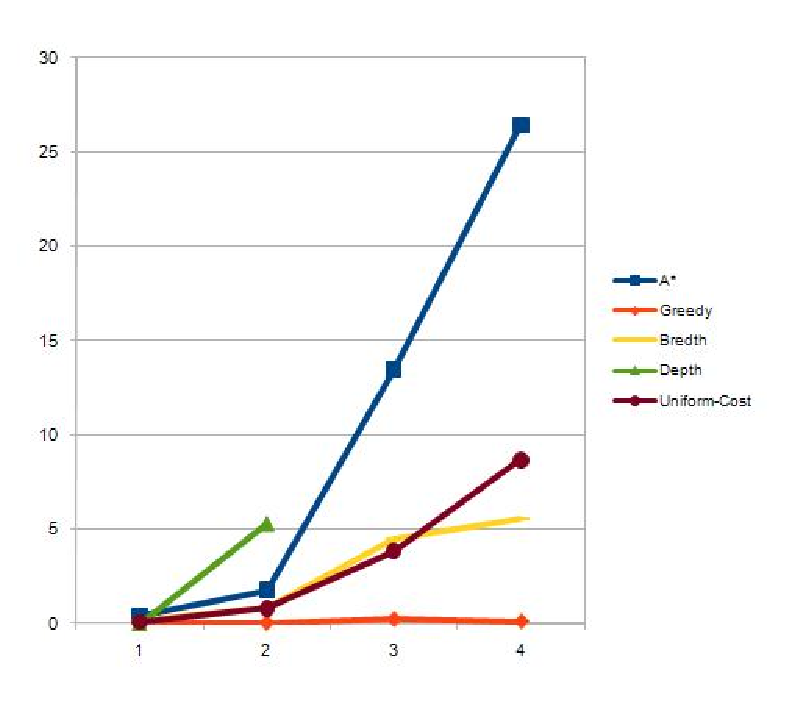
\includegraphics[width=6in]{resultats-planif} %ou image.png, .jpeg etc.
\caption{Progression du temps de calcul pour différents algorithmes pour différents environnements} 
\end{figure}

Avec ces résultats nous pouvons voir l'évolution des algorithmes. Nous avons doublé la distance entre le joueur et son but pour chaque environnement. Nous pouvons ainsi voir un estimé de la complexité de chacune des algorithmes.

En première considération, la technique de profondeur d'abord est un algorithme vraiment risqué. Cette technique dépasse rapidement la mémoire maximale permise à l'environnement prolog. Cette technique est donc à éviter. Il semble que l'algorithme s'étant trop dans une branche dans l'environnement 2, 3 et 4.

En second considération, la technique A* s'emballe plus le but s'éloigne. Nous pouvons voir que le A* effectue beaucoup plus de calculs que n'importe quelle autre solution. L'algorithme utilise une queue avec priorité tout comme la méthode Avare ainsi que la méthode à coût uniforme. Cependant, elle tient compte de plus de paramètres que ces derniers; elle tient compte de chacun des paramètres utilisés par ces derniers. Le fait d'utiliser deux éléments dans le coût total pour l'insertion dans la queue fait que beaucoup de changement de branche est effectué.

En troisième considération, lorsque le but est très loin, seul l'algorithme avare réussit à résoudre le problème.

Avec toutes ces considérations, nous suggérons l'utilisation de la méthode avare.



\section{Representation STRIPS ou ADL des actions possibles de BlockBlitz}
% Erick 
% 1.5 pages
Par souci de concision et de lisibilité, l'environnement de jeu initial et l'environnement de jeu final seront omis des paramètres, des préconditions et des effets des actions présentées bien qu'ils soient utilisés de fa\c con explicite dans le programme remis.  Pour l'ensemble des actions présentées, nous assumerons un environnement de jeu composé des faits suivants, les multiplicités présentées représentent le nombre de faits distincts du type présenté pouvant être retrouvés dans l'environnement, ex: nbJoueur(N), 1 signifie qu'un seul fait de type nbJoueur est présent dans l'environnement et block(...), 1+ signifie que chaque bloc est représenté par son propre fait et qu'il y en a autant que de blocs.

\begin{center}
  \begin{tabular}{@{} ccc @{}}
    \hline
    Fait & Multiplicité & Signification \\ 
    \hline
    NbJoueur(n) & 1 & $n$ est le nombre de joueurs \\ 
    NbBlock(n) & 1 & $n$ est le nombre de blocks \\ 
    NbColonnes(n) & 1 & $n$ est le nombre de colonnes \\ 
    NbRangees(n) & 1 & $n$ est le nombre de rangées \\ 
    Block(id,x,y) & 1+ & $id$ est la valeur du block, \\
                                  && $x$ est la position en selon $x$ \\
                                  && et $y$ est la position selon $y$ \\ 
    Player(id,nom,x,y,blockId) & 1+ & $id$ est l'identifiant unique du joueur \\
                                                              && $nom$ est le nom assigné au joueur \\ 
                                                              && $x$ est la position selon $x$ \\
                                                              && $y$ est la position selon $y$ \\
                                                              && $blockId$ est l'identifiant du bloc possédé par le joueur\\
    Nom(nom) & 1 & $nom$ est le nom du joueur \\ 
    \hline
  \end{tabular}
\end{center}

En plus de ces faits de base, les prédicats suivants sont utilisés pour faciliter l'expression des préconditions et des effets. \\
\\
Il est nécessaire de traduire la direction en coordonnées. Pour ce faire, le prédicat $Direction(posx,posy,newx,newy,direction)$ est utilisé pour déterminer la nouvelle position du joueur à partir de sa position précédente.  Il y a huit entrées pour chacune des direction.  L'entrée pour la direction $1$ est la suivante, les autres entrées sont laissées comme exercice au lecteur.
\begin{equation*}
	Direction(posx,posy,newx,newy, 1) \Leftarrow newy = posy + 1 \wedge newx = posx 
\end{equation*}

Les deux derniers prédicats sont les suivants.  $Empty(posx,posy)$ assure que la case visée ne contient rien, c'est-à-dire aucun joueur ou bloc, et $Exist(posx,posy)$ valide que la case visée appartient bel et bien à l'environnement, c'est-à-dire qu'elle est contenue dans ses limites.
\begin{eqnarray*}
	Empty(posx,posy) \Leftarrow & \lnot Block(\_,posx,posy)  \wedge \lnot Player(\_,\_,posx,posy,\_) \\
	Exist(posx,posy) \Leftarrow & posx  \geq 0 \wedge posy \geq 0 \\
	                                                    \wedge & NbColonnes(nbColonnes)  \wedge NbRangees(nbRangees) \\
	                                                   \wedge & posx < nbColonnes \wedge posy < nbRangees 
\end{eqnarray*}

Il est alors très aisé d'exprimer les préconditions et les effets de chacune des actions.

\begin{tabbing}
\textit{Action}\=\textit{(Move(direction))}\=,\\
\> PRECOND: \> $Nom(nom) \wedge Player(id,nom,posx,posy,blockid)$ \\ 
\> \> $  \wedge \ Direction(posx,posy,newx,newy,direction) $ \\
\> \> $   \wedge \ Exist(newx,newy) \wedge Empty(newx,newy) $ \\               
\> EFFECT: \>$ \lnot Player(id,nom,posx,posy,blockid) $ \\
\>  \> $\wedge\ Player(id,nom,newx,newy,blockid)$ .\\
\end{tabbing}

Pour le cas où le joueur ne possède pas de bloc, l'action $take$ est la suivante:

\begin{tabbing}
\textit{Action}\=\textit{(Take(direction))}\=,\\
\> PRECOND: \> $Nom(nom) \wedge Player(id,nom,posx,posy,0)$ \\ 
\> \> $  \wedge \ Direction(posx,posy,newx,newy,direction) $ \\
\> \> $   \wedge \ Exist(newx,newy) \wedge Block(newblockid,newx,newy) $ \\               
\> EFFECT: \>$ \lnot Player(id,nom,posx,posy,0) $ \\
\>  \> $\wedge\ Player(id,nom,newx,newy,newblockid)$ \\
\> \> $\wedge\ \lnot Block(newblockid,newx,newy) $ .\\
\end{tabbing}

Pour le cas où le joueur possède déjà un bloc, l'action $take$ est plutôt:
\begin{tabbing}
\textit{Action}\=\textit{(Take(direction))}\=,\\
\> PRECOND: \> $Nom(nom) \wedge Player(id,nom,posx,posy,blockid)$ \\ 
\> \> $  \wedge \ Direction(posx,posy,newx,newy,direction) $ \\
\> \> $   \wedge \ Exist(newx,newy) \wedge Block(newblockid,newx,newy) $ \\               
\> EFFECT: \>$ \lnot Player(id,nom,posx,posy,blockid) $ \\
\>  \> $\wedge\ Player(id,nom,newx,newy,newblockid)$ \\
\> \> $\wedge\ \lnot Block(newblockid,newx,newy) $ \\
\> \> $\wedge\ Block(blockid,newx,newy) $ .\\
\end{tabbing}

\begin{tabbing}
\textit{Action}\=\textit{(Drop(direction))}\=,\\
\> PRECOND: \> $Nom(nom) \wedge Player(id,nom,posx,posy,blockid)$ \\ 
\> \> $  \wedge \  \lnot Player(id,nom,posx,posy,0) $ \\
\> \> $  \wedge \ Direction(posx,posy,newx,newy,direction) $ \\
\> \> $   \wedge \ Exist(newx,newy) \wedge Empty(newx,newy) $ \\               
\> EFFECT: \>$ \lnot Player(id,nom,posx,posy,blockid) $ \\
\>  \> $\wedge\ Player(id,nom,posx,posy,0)$ \\
\> \> $\wedge\ Block(blockid,newx,newy) $ .\\
\end{tabbing}

Bien que la problématique présente deux cas distincts pour l'attaque, avec la représentation proposée, la même description s'applique dans les deux cas (joueur possède ou non un bloc).  De plus, pour fins de planification, nous allons considérer que l'action réussi toujours.:

\begin{tabbing}
\textit{Action}\=\textit{(Attack(direction))}\=,\\
\> PRECOND: \> $Nom(nom) \wedge Player(id,nom,posx,posy,blockid)$ \\ 
\> \> $  \wedge \ Direction(posx,posy,newx,newy,direction) $ \\
\> \> $  \wedge \ Player(id2,nom2,newx,newy,blockid2) $ \\
\> \> $  \wedge \ \lnot Player(id2,nom2,newx,newy,0) $ \\
\> \> $ \wedge\ \lnot Block(bid,newx,newy) \wedge \ Exist(newx,newy)$ \\               
\> EFFECT: \>$ \lnot Player(id,nom,posx,posy,blockid) $ \\
\>  \> $\wedge\ Player(id,nom,posx,posy,blockid2)$ \\
\>  \> $\wedge\ \lnot Player(id2,nom2,newx,newy,blockid2)$ \\
\>  \> $\wedge\ Player(id2,nom2,newx,newy,blockid)$ .\\
\end{tabbing}

Finalement, l'action $None$ ne possède aucune précondition et n'a aucun effet sur l'environnement.

\section{Description et une explication du vocabulaire des parties principales de la solution}
À haut niveau, notre programme comporte 3 grandes sections:
\begin{itemize}
	\item Une représentation des actions, leur préconditions et leurs effets sur l'environnement
	\item Un algorithme de recherche utilisant les actions, un environnement et un but pour déterminer une séquence d'actions permettant d'atteindre le but
	\item Des prédicats de planification ajustant le comportement du joueur en fonction de l'état courant de l'environnement
\end{itemize}

La représentation des actions a été abordée à la section précédente.  Pour la recherche, voici les éléments les plus importants. 

L'expansion des actions possibles est réalisée en trouvant chacune des actions pouvant s'appliquer sur l'environnement.  Ce test est réalisé à l'aide du prédicat Action.
\begin{equation}
	successors = { \forall action Action(action, env) } \Rightarrow Expand( node(env, action), successors)
\end{equation}
Un exemple du prédicat $Action$ pour l'action $move$:
\begin{equation}
        \forall direction, env Move(direction, env) \Rightarrow Action(Move(direction), env)
\end{equation}

La validation du but est réalisée en testant que le joueur possède effectivement un bloc, assumant que le $nom$ est le nom du joueur.  Le prédicat $Player(nom,positionX,positionY,block)$ détermine si un joueur ayant un $nom$ à la position $positionX$ et $positionY$ et un $block$ existe, l'environnement est ici implicite:
\begin{eqnarray*}
	\forall & positionX, positionY\ \exists block Player(nom,positionX,positionY, block) \\
	 \wedge & block != 0 \Rightarrow ButAtteint(nom)
\end{eqnarray*}

La recherche peut etre résumée, en disant qu'il existe une solution telle que le plan $Plan$ généré par cette solution est valide, que l'état donné par le dernier noeud $node$ n'a pas été visité avant, qu'il s'agit du noeud minimisant le coût et que le but est atteint:
\begin{eqnarray*}
	\exists & solution\ Plan(solution) \wedge EtatNonVisite(fringe) \wedge MoindreCout(fringe,node) \\  \wedge &  ButAtteint \Rightarrow RechercheGraphe(fringe, solution, closedSet)
\end{eqnarray*}

Finalement, pour la planification, en autant que le plan soit toujours valide nous retournons la prochaine action, dans les autres cas un autre plan est établi.  Lorsque le but est atteint, l'action $none$ est retournée tant que le but est satisfait par l'environnement.


\section{Description de parties principales de notre solution}
% Alex
% 1 page
La particularité principale que nous avons implémentée dans notre solution est la méthode généralisée du parcours de graphe. Tout en respectant les méthodes de la logique de premier ordre, nous avons transcrit littéralement l'algorithme. C'est-à-dire que nous ne forçons pas une structure de donnée à l'intérieur de l'algorithme. Nous avons procédé ainsi puisque cet algorithme est noyau de toutes les méthodes de recherches que nous avons utilisées (\textit{profondeur d'abord, largeur d'abord, coût uniforme, avare et A*}). C'est d'ailleurs ainsi que nous sommes parvenus à comparer rapidement les performances de ces cinq techniques.

Voici les structures de données que nous avons utilisées dans notre implémentation de planification.

\begin{itemize}
\item \textbf{Node} : \textit{node(Etat,NoeudParent,Action,Profondeur,Cout)}
\item \textbf{Action} : \textit{action(Action,Etat, Cout, EtatResultant, CoutResultant)}
\end{itemize}

Le \textbf{Node} est l'élément qui représente le graphe que l'algorithme de recherche parcours. L'\textbf{Action}, tel que présenté à la section de la représentation STRIPS des actions possible de \textit{BlockBlitz}, valide d'abord si le mouvement peut être effectué sur l'environnement. Nous avons cependant explicitement partagé un environnement au lieu d'utiliser la base de connaissance de l'interpréteur prolog. L'environnement est représenté par la variable \textit{Etat}. De plus, si l'action est effectivement valide, nous retournons l'environnement résultant ainsi que le nouveau coût qui est relié au parcours effectué.

Avec notre représentation, nous avons pu effectuer l'expansion de nos noeuds lors du parcours de graphe de façon efficace. Dans le cas de \textit{BlockBlitz}, l'expansion signifie de trouver la prochaine action à effectuer. Nous avons donc utilisé la fonction \textit{findall} avec comme objectif le prédicat avec seulement l'état et le coût comme variable assignée. Cela nous donne alors la liste des noeuds successeurs avec leur nouvel environnement déjà construit ainsi que le cout de l'action. C'est la fonction \textit{findall} qui, avec l'inférence et le fait de trouver une action valide, retourne le nouveau cout et l'environnement résultant et l'ajoute à la liste résultante.


\section{Recommandation de la pertinence des méthodes d'algorithmes évolués}
% Alex
% 1 page

% Planification continuelle, multiagent, conditionnelle
Dans le cadre de notre analyse, nous avons également survolé des techniques de planification plus évoluées, c'est-à-dire des techniques pour lesquelles les hypothèses sur l'environnement de jeu sont moins restrictives.  La recherche classique tel qu'envisagé précédemment assume que l'environnement est pleinement observable, statique et déterministe et que les actions affectant l'environnement sont correctes et complètes. Ces hypothèses permettent de réaliser la planification beaucoup plus simplement.
Dans le cas du jeu \textit{BlockBlitz}, pour que l'IA se comporte de fa\c con optimale, ces hypothèses sont trop restrictives puisque nous n'avons pas affaire à un environnement statique, non-déterministe lors d'attaques et nous sommes en présence d'autres agents compétiteurs.  Il est donc pertinent d'évaluer les techniques de planification plus avancées.  Les caractéristiques de chacune de ces techniques sont brièvement abordées ci-après ainsi que leur applicabilité au jeu \textit{BlockBlitz}.

\subsection{Planification conditionnelle}
La planification conditionnelle tente de gérer l'incertitude liée à un environnement non déterministe en vérifiant à différents points du plan que certaines conditions sont vraies et tente d'apporter un plan de contingence pour les différents scénarios possibles de sorte que pour toutes les situations possibles le plan sera accompli.

Dans notre cas, la planification conditionnelle pourrait être intéressante puisque les actions d'attaque sont non-déterministes. Nous aurions alors pu créer un plan pour chaque possibilité d'attaque afin que le but soit atteint dans tous les cas.

\subsection{Replanification et observation de l'exécution du plan}
La replanification consiste à vérifier au fur et à mesure de l'exécution du plan que celui-ci est encore valide.  Cela peut être fait une action à la fois ou bien pour l'ensemble du plan à chaque étape.  Lorsque les conditions d'applicabilité du plan ne sont plus valides, il est alors possible d'en générer un nouveau. Cela est très approprié dans le cas d'un environnement dynamique.

Cette technique est parfaitement applicable au jeu \textit{BlockBlitz}, et nous l'avons d'ailleurs utilisée avec succès puisque la présence d'autres agents dans le jeu modifie l'environnement pendant l'exécution du plan, le rendant dynamique.  Nous validons à chaque tour la validité du plan avant de fournir la prochaine action.

\subsection{Planification multiagent}

La planification multi-agents tient compte des autres agents actifs dans l'environnement pour l'établissement des plans.  Dans le cas du jeu \textit{BlockBlitz}, il s'agit d'une situation compétitive où les autres agents tentent d'accomplir leur(s) but(s) au détriment ou non de leurs adversaires.  Pour être utilisable, l'IA doit générer des plans pour les autres joueurs et en tenir compte dans l'établissement de son propre plan.  Cela rend la complexité de la recherche beaucoup plus importante et implique un domaine de recherche nommé la théorie des jeux.  Étant donné la complexité cela n'a pas été abordé dans le cadre de cette analyse.  

Cependant, pour réaliser un IA convainquant et intéressant pour le jeu il est nécessaire que celui-ci applique ce type de technique et dans le cadre d'une stratégie de développement de jeu plus global cela vaudrait la peine de s'attarder à comprendre et appliquer cette technique.


\section{Conclusion}
% Alex
% 0.5 page


\end{document}
